% Options for packages loaded elsewhere
% Options for packages loaded elsewhere
\PassOptionsToPackage{unicode}{hyperref}
\PassOptionsToPackage{hyphens}{url}
\PassOptionsToPackage{dvipsnames,svgnames,x11names}{xcolor}
%
\documentclass[
  letterpaper,
  DIV=11,
  numbers=noendperiod]{scrartcl}
\usepackage{xcolor}
\usepackage[margin=1in]{geometry}
\usepackage{amsmath,amssymb}
\setcounter{secnumdepth}{5}
\usepackage{iftex}
\ifPDFTeX
  \usepackage[T1]{fontenc}
  \usepackage[utf8]{inputenc}
  \usepackage{textcomp} % provide euro and other symbols
\else % if luatex or xetex
  \usepackage{unicode-math} % this also loads fontspec
  \defaultfontfeatures{Scale=MatchLowercase}
  \defaultfontfeatures[\rmfamily]{Ligatures=TeX,Scale=1}
\fi
\usepackage{lmodern}
\ifPDFTeX\else
  % xetex/luatex font selection
\fi
% Use upquote if available, for straight quotes in verbatim environments
\IfFileExists{upquote.sty}{\usepackage{upquote}}{}
\IfFileExists{microtype.sty}{% use microtype if available
  \usepackage[]{microtype}
  \UseMicrotypeSet[protrusion]{basicmath} % disable protrusion for tt fonts
}{}
\makeatletter
\@ifundefined{KOMAClassName}{% if non-KOMA class
  \IfFileExists{parskip.sty}{%
    \usepackage{parskip}
  }{% else
    \setlength{\parindent}{0pt}
    \setlength{\parskip}{6pt plus 2pt minus 1pt}}
}{% if KOMA class
  \KOMAoptions{parskip=half}}
\makeatother
% Make \paragraph and \subparagraph free-standing
\makeatletter
\ifx\paragraph\undefined\else
  \let\oldparagraph\paragraph
  \renewcommand{\paragraph}{
    \@ifstar
      \xxxParagraphStar
      \xxxParagraphNoStar
  }
  \newcommand{\xxxParagraphStar}[1]{\oldparagraph*{#1}\mbox{}}
  \newcommand{\xxxParagraphNoStar}[1]{\oldparagraph{#1}\mbox{}}
\fi
\ifx\subparagraph\undefined\else
  \let\oldsubparagraph\subparagraph
  \renewcommand{\subparagraph}{
    \@ifstar
      \xxxSubParagraphStar
      \xxxSubParagraphNoStar
  }
  \newcommand{\xxxSubParagraphStar}[1]{\oldsubparagraph*{#1}\mbox{}}
  \newcommand{\xxxSubParagraphNoStar}[1]{\oldsubparagraph{#1}\mbox{}}
\fi
\makeatother


\usepackage{longtable,booktabs,array}
\usepackage{calc} % for calculating minipage widths
% Correct order of tables after \paragraph or \subparagraph
\usepackage{etoolbox}
\makeatletter
\patchcmd\longtable{\par}{\if@noskipsec\mbox{}\fi\par}{}{}
\makeatother
% Allow footnotes in longtable head/foot
\IfFileExists{footnotehyper.sty}{\usepackage{footnotehyper}}{\usepackage{footnote}}
\makesavenoteenv{longtable}
\usepackage{graphicx}
\makeatletter
\newsavebox\pandoc@box
\newcommand*\pandocbounded[1]{% scales image to fit in text height/width
  \sbox\pandoc@box{#1}%
  \Gscale@div\@tempa{\textheight}{\dimexpr\ht\pandoc@box+\dp\pandoc@box\relax}%
  \Gscale@div\@tempb{\linewidth}{\wd\pandoc@box}%
  \ifdim\@tempb\p@<\@tempa\p@\let\@tempa\@tempb\fi% select the smaller of both
  \ifdim\@tempa\p@<\p@\scalebox{\@tempa}{\usebox\pandoc@box}%
  \else\usebox{\pandoc@box}%
  \fi%
}
% Set default figure placement to htbp
\def\fps@figure{htbp}
\makeatother





\setlength{\emergencystretch}{3em} % prevent overfull lines

\providecommand{\tightlist}{%
  \setlength{\itemsep}{0pt}\setlength{\parskip}{0pt}}



 


\usepackage{booktabs}
\usepackage{longtable}
\usepackage{array}
\usepackage{multirow}
\usepackage{wrapfig}
\usepackage{float}
\usepackage{colortbl}
\usepackage{pdflscape}
\usepackage{tabu}
\usepackage{threeparttable}
\usepackage{threeparttablex}
\usepackage[normalem]{ulem}
\usepackage{makecell}
\usepackage{xcolor}
\KOMAoption{captions}{tableheading}
\usepackage{sectsty}
\usepackage{xcolor}
\usepackage{fancyhdr}
\definecolor{wdlblue}{HTML}{012D4A}
\definecolor{wdlteal}{HTML}{00A7B5}
\sectionfont{\color{wdlblue}\uppercase}
\subsectionfont{\color{wdlblue}}
\usepackage{etoolbox}
\makeatletter
\patchcmd{\@sect}{\fi#7}{\fi\color{wdlteal}\hrule height 1.5pt \kern 3pt\color{black}#7}{}{}
\makeatother
\pagestyle{fancy}
\makeatletter
\@ifpackageloaded{caption}{}{\usepackage{caption}}
\AtBeginDocument{%
\ifdefined\contentsname
  \renewcommand*\contentsname{Table of contents}
\else
  \newcommand\contentsname{Table of contents}
\fi
\ifdefined\listfigurename
  \renewcommand*\listfigurename{List of Figures}
\else
  \newcommand\listfigurename{List of Figures}
\fi
\ifdefined\listtablename
  \renewcommand*\listtablename{List of Tables}
\else
  \newcommand\listtablename{List of Tables}
\fi
\ifdefined\figurename
  \renewcommand*\figurename{Figure}
\else
  \newcommand\figurename{Figure}
\fi
\ifdefined\tablename
  \renewcommand*\tablename{Table}
\else
  \newcommand\tablename{Table}
\fi
}
\@ifpackageloaded{float}{}{\usepackage{float}}
\floatstyle{ruled}
\@ifundefined{c@chapter}{\newfloat{codelisting}{h}{lop}}{\newfloat{codelisting}{h}{lop}[chapter]}
\floatname{codelisting}{Listing}
\newcommand*\listoflistings{\listof{codelisting}{List of Listings}}
\makeatother
\makeatletter
\makeatother
\makeatletter
\@ifpackageloaded{caption}{}{\usepackage{caption}}
\@ifpackageloaded{subcaption}{}{\usepackage{subcaption}}
\makeatother
\usepackage{bookmark}
\IfFileExists{xurl.sty}{\usepackage{xurl}}{} % add URL line breaks if available
\urlstyle{same}
\hypersetup{
  pdftitle={Predicting new COVID-19 cases in the US: A Comparison of a Compatmental model (SIR) and XGBOOST Machine Learning Model},
  pdfauthor={Basil Okola},
  colorlinks=true,
  linkcolor={blue},
  filecolor={Maroon},
  citecolor={Blue},
  urlcolor={Blue},
  pdfcreator={LaTeX via pandoc}}


\title{Predicting new COVID-19 cases in the US: A Comparison of a
Compatmental model (SIR) and XGBOOST Machine Learning Model}
\author{Basil Okola}
\date{February 11, 2026}
\begin{document}
\maketitle
\begin{abstract}
\textbf{Background}: Figuring out the number of new COVID-19 cases was
key in aligning interventions to hotspots. This included ensuring there
were enough beds for admissions, key protection gear like face masks,
oxygen supply and intensive care unit space. A lot of mechanistic models
were build borrowing from the traditional SIR model. Additionally,
researchers explored machine learning techniques to predict the course
of the infections.

\textbf{Methods}: In this report, we compare the performance of a SIR
model to an XGBOOST prediction model in predicting new cases in each of
the American states, 3 years after the pandemic.

\textbf{Results}: The XGBOOST ML approach demonstrated robust
goodness-of-fit, effectively capturing the non-linear peak dynamics
across varying geographic replicates.
\end{abstract}


\section{Introduction}\label{introduction}

We chose to use data on COVID-19 cases assembled by a team from
\href{https://vac-lshtm.shinyapps.io/ncov_tracker/\#}{The London School
of Health \& Tropical Medicine}

Model comparisons

\pandocbounded{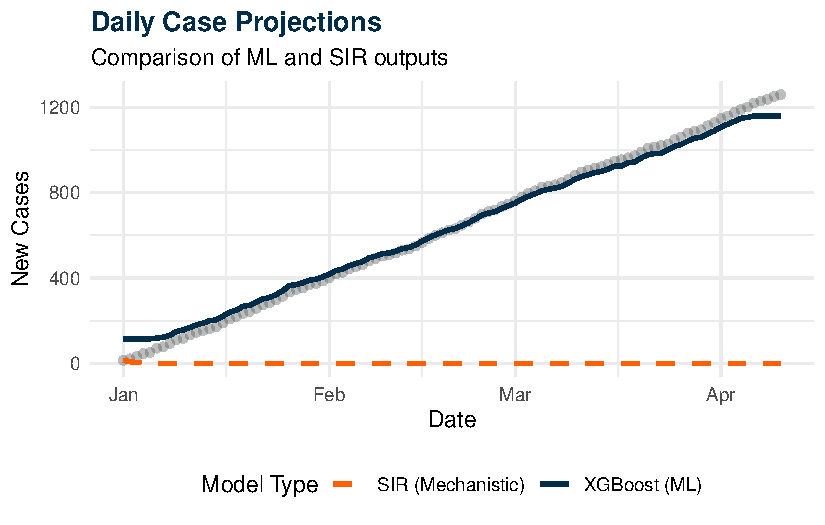
\includegraphics[keepaspectratio]{aphrc-report_files/figure-pdf/unnamed-chunk-2-1.pdf}}

Summary of parameters

\begin{table}[!h]
\centering
\caption{\label{tab:unnamed-chunk-3}SIR Model Parameters}
\centering
\begin{tabular}[t]{>{}l>{}r}
\toprule
\cellcolor[HTML]{012d4a}{\textcolor{white}{\textbf{Parameter}}} & \cellcolor[HTML]{012d4a}{\textcolor{white}{\textbf{Value}}}\\
\midrule
\textcolor[HTML]{012d4a}{\textbf{\cellcolor{gray!10}{Beta (Transmission)}}} & \textcolor[HTML]{FF5F00}{\textbf{\cellcolor{gray!10}{0.1869}}}\\
\textcolor[HTML]{012d4a}{\textbf{Gamma (Recovery)}} & \textcolor[HTML]{FF5F00}{\textbf{0.8036}}\\
\textcolor[HTML]{012d4a}{\textbf{\cellcolor{gray!10}{Basic Reproduction (R0)}}} & \textcolor[HTML]{FF5F00}{\textbf{\cellcolor{gray!10}{0.2325}}}\\
\bottomrule
\end{tabular}
\end{table}

Simulations

\begin{table}[!h]
\centering
\caption{\label{tab:unnamed-chunk-5}Global Assessment Metrics}
\centering
\begin{tabular}[t]{rr}
\toprule
\cellcolor[HTML]{012d4a}{\textcolor{white}{rmse}} & \cellcolor[HTML]{012d4a}{\textcolor{white}{mape}}\\
\midrule
1.460515 & 99.80213\\
\bottomrule
\end{tabular}
\end{table}

\pandocbounded{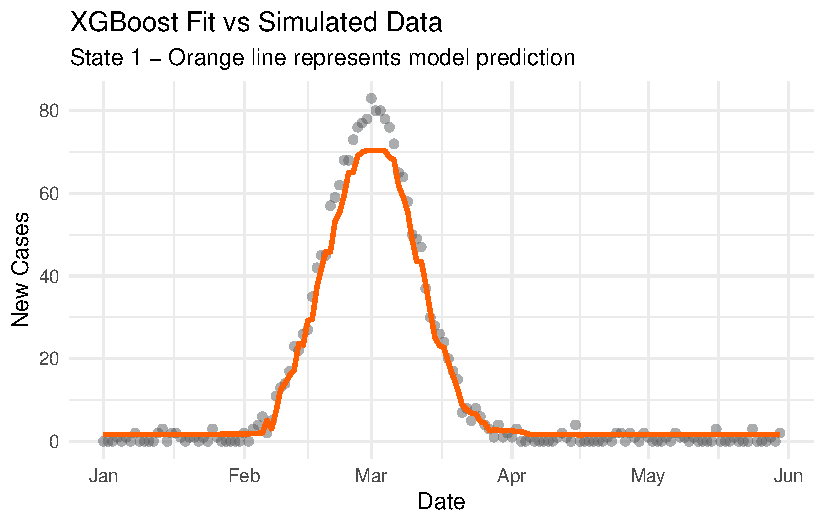
\includegraphics[keepaspectratio]{aphrc-report_files/figure-pdf/unnamed-chunk-5-1.pdf}}




\end{document}
